% This is a comment
\documentclass[journal]{IEEEtran}
% IEEEtran.cls must be in the same folder.
% If not, manually specify the path to it like:
% \documentclass[conference]{../sty/IEEEtran}

% This is the somewhat "standard" set of packages that I typically include in all my documents. Some of them probably aren't actually used, so it isn't "pretty" but it gets the job done.
\usepackage{array}
\usepackage{url}
\usepackage{epsf}
\usepackage{verbatim}
\usepackage{morefloats}
\usepackage{flushend}
\usepackage[cmex10]{amsmath}
\usepackage{esint}
\usepackage{amssymb}
\usepackage{graphicx}
\usepackage{hhline}
\usepackage{longtable}
\usepackage{rotating}
\usepackage{lscape}
\usepackage{psfrag}
\usepackage[labelformat=simple]{subcaption}
\renewcommand\thesubfigure{(\alph{subfigure})} % makes subfigure labels appear as (a) and (b) and referenced like this in the text
\usepackage{epstopdf}
\usepackage{cite}
\usepackage{booktabs} %professional-looking tables
\usepackage{multicol} %used for getting multicolumn without page-break
\usepackage{multirow} %used for multi row in tables
\usepackage{setspace}
\usepackage[dvipsnames]{xcolor}
\usepackage{mathtools}
\usepackage{textcomp}
\newcommand{\textapprox}{\raisebox{0.5ex}{\texttildelow}} % defines a new command to make the ~ in text to denote "approximately"


% I like to keep my images that I will include as figures organized in a subfolder names "figures". 
% Adjust this appropriately for your use by either changing the path or by commenting it out if you just want to leave all the figures in the same folder as your main file.
\graphicspath{{./figures/}} 


\begin{document}
% paper title
% can use linebreaks \\ within to get better formatting as desired
% Generally good to not put math or special symbols in the title.
\title{Approximating the Capacitance of Square Plates: A Method of Moments Convergence Study}

% I'm mashing some templates together here. If you write an actual IEEE transactions paper in LaTeX start from their template and then modify things like packages and files you want to include from there as opposed to starting from this document provided in this course.
\author{
\IEEEauthorblockN{Samuel J. Wyss\IEEEauthorrefmark{2} }
\IEEEauthorblockA{\\ \IEEEauthorrefmark{2}School of Nuclear Engineering\\
Purdue University\\
West Lafayette, Indiana 47907 \\ E-mail: wysss@purdue.edu}\\
}

% make the title area
\maketitle

% As a general rule, do not put math, special symbols or citations
% in the abstract
\begin{abstract}
The Method of Moments (MoM) is applied to simulate the capacitance of an arbitrarily sized, square metallic plate. To model this system \textit{in silico}, the Electrostatic Integral Equation (EIE) is used to simulate the charge distribution for a fixed potential on the metallic plate. The total charge is then determined by integrating element-wise over the surface which is then used to solve for plate capacitance. This procedure is used to evaluate various formulations of the underlying integral equations from approximations of square elements, exact forms, to subdomain collocation. Capacitance values from these methods are first compared to data found in the literature as a verification and validation step and then compared to each other in terms of the mesh size required, and corresponding asymptotic number of operations, for these methods to achieve convergence.
\end{abstract}

% For peerreview papers, this IEEEtran command inserts a page break and
% creates the second title. It will be ignored for other modes.
\IEEEpeerreviewmaketitle

% the \input command allows you to tell the compiler to go through the .tex file placed in the command. Breaking out your main sections of the paper in this way helps keep the code/tex document more organized typically.
%\section{Getting Started}
\label{sec:getting-started}
Before you can start using LaTeX you need to get your computer set up for it. If you don't want to go through the process of installing a few different programs on your computer, you can sign up to use Overleaf. This is an online LaTeX editor that Purdue students and faculty have access to for free. It is fairly easy to use and has nice features to enable collaborating on documents.

If you want to use LaTeX on your computer, you first need to install MiKTeX. If you google it you should be able to quickly find the download instructions. Once you have that installed, I recommend using an additional ``editor'' on top of that which has additional features to improve the usability. I personally use TeXstudio because that is what was recommended to me initially and I haven't spent any time shopping around for a different tool because it seems straightforward and capable enough.

Note that I am using the IEEE template for formatting in this document. You can easily swap to a different journal's template by substituting in their class file (replacing the IEEEtran file with something else) and making a few other edits to the main TeX document. This kind of swap can be a little tedious, but it is typically substantially easier than trying to swap between two Word document templates from different journals. I will say that the IEEE template can be a little annoying with formatting when the document you are writing only has a small amount of content in it. It usually starts to do a better job once the document gets filled in more, but if you have lots of long equations it can still struggle. These issues are why there is occasionally some weird spacing between certain sections in this document. LaTeX is doing its best to try and move things around on the pages to make it look good and match the IEEE format, but sometimes more control of these issues can be needed. I usually leave this to the editorial staff at a journal to fix, since they are going to mess with whatever you submit most of the time anyway.
\section{Introduction}
\label{sec:intro}

Contrary to many other methods in Computational Electromagnetics (CEM), the Method of Moments (MoM) is purely based on the integral form of Maxwell's Equations and underlying Green's Functions \cite{rothlecnotes}, \cite{jin2011theory}. In the context of the Electrostatic Integral Equation (EIE), MoM uses the potential contributed by individual point charges on surface elements to solve for charge density as a function of location. This charge distribution can trivially be integrated over surface elements to solve for the net charge on an surface for an arbitrary geometry and applied potential. From this, the capacitance of said structure can easily be obtained.

In matrix form, the EIE relates the point source response of charges in a given surface element to all other surface elements and the applied potential. The use of Green's Functions in the problem formulation allows for these problems to be solved without the need to spatially terminate the simulation region which is a common source of error in other CEM methods. However, the use of Green's Functions results in fully dense matrices, thus requiring the computational complexities and memory footprint that comes with solving them which at first may be seen as a downside of MoM. However, these matrices only require the discretization of surfaces \cite{rothlecnotes}, \cite{jin2011theory} thereby resulting in much smaller system matrices overall which helps to compensate for the typical $O(n^3)$ computation complexity required to solve these dense systems. 

The development and results of this work are laid out as follows. Section \ref{sec:mathmod} contains a short derivation of the EIE from Gauss's Law followed by the setup of the EIE matrix equations for a circular approximation of square surface elements, an exact form for square surface elements, and finally the subdomain collocation. Section \ref{sec:numres} contains a verification of the model with a capacitance range found in the literature, an explanation of the plate charge distribution, and finally, an analysis of the asymptotic number of operations required to determine the plate capacitance for all three methods. Finally, Section \ref{sec:conclusion} contains closing remarks regarding the analysis and potential future work.
\section{Mathematical Model}
\label{sec:mathmod}

To model these systems \textit{in silico}, an appropriate mathematical model must first be derived from Maxwell's Equations. The development of said model is arranged as follows. Section \ref{subsub:eie} contains the derivation of the EIE from Maxwell's Equations followed by surface element discretization into a simultaneous set of equations. Section \ref{subsub:mat-approx} outlines three formulations of the Systems matrix $A$ starting with elements approximated as circles, an exact solution, and finally subdomain collocation. 

\subsubsection{The Electrostatic Integral Equation (EIE)}
\label{subsub:eie}
From basic electrostatics, the integral form of Gauss's Equation over some surface $S$ is as follows
\begin{align}
    \iint_S\epsilon_0^{-1}g(\textbf{r},\textbf{r'})\rho_s(\textbf{r'})dS'=\Phi(r)
\end{align}
where $\epsilon_0$ is the permittivity of free space, $\rho_s(\textbf{r'})$ is the surface charge density, $\Phi(r)$ is the electrostatic potential, and $g(\textbf{r},\textbf{r'})$ is the corresponding Green's function (integration kernel)
\begin{align}
    g(\textbf{r},\textbf{r'})=\frac{1}{4\pi|\textbf{r}-\textbf{r'}|}
\end{align}

\subsubsection{System Matrix Approximations}
\label{subsub:mat-approx}





\section{Numerical Results}
\label{sec:numres}
With the mathematical model now fully established, the implementation of this model is documented in Section \ref{subsec:impl}. From here Sections \ref{subsec:vv} verifies the model against exact dispersion relations for multiple modes in rectangular waveguides. Section \ref{subsec:circ_guides} performs an analysis of Dispersion characteristics in circular waveguides and addresses the advantages of using FEA for this task. Finally, Section \ref{subsec:rid_guides} compares the dispersion characteristics of the rectangular and ridged rectangular waveguides for multiple modes and discusses practical applications of ridged waveguides.

\subsection{Implementation}
\label{subsec:impl}
All meshes used in the following sections were generated using Coreform Cubit \cite{cubit} with a tutorial provided by \cite{rothlecnotes}. For the rectangular waveguide found in \ref{subsec:vv}, a WR-90, X-band waveguide with $a=0.02286$m and $b=0.01016$m was used \cite{everythingrf}. For the circular waveguide used in \ref{subsec:circ_guides}, a similarly sized circular waveguide of radius $r=0.01$m was used. In order to compare the non-ridged to the ridged waveguide the same WR-90, X-band waveguide was used in Section \ref{subsec:rid_guides} as in Section \ref{subsec:vv}; however, with two $0.0025\times0.0025$m notches cut out along the long edge. Example meshes of the later two geometries can be found in Figures \ref{fig:circular_guide}-\ref{fig:ridged_guide}. These meshes were generated using Coreform Cubit's \verb|TriAdvance| algorithm all containing $\approx2000$ nodes which is appropriate for the applications studied here. Coreform Cubit's \verb|nodeset| feature was used to create a set of all nodes on the boundaries of these geometries. This allows for $O(1)$ lookups of elements on the boundary which was utilized heavily when performing TM mode analysis. These meshes were saved into the ABAQUS \verb|.inp| ASCII format, which was chosen for its human readability which was invaluable during the development of this code.

\begin{figure}[h!]  
	\centering
	%the command within the [] sets the width of the figure, stability-condition is the jpg name
	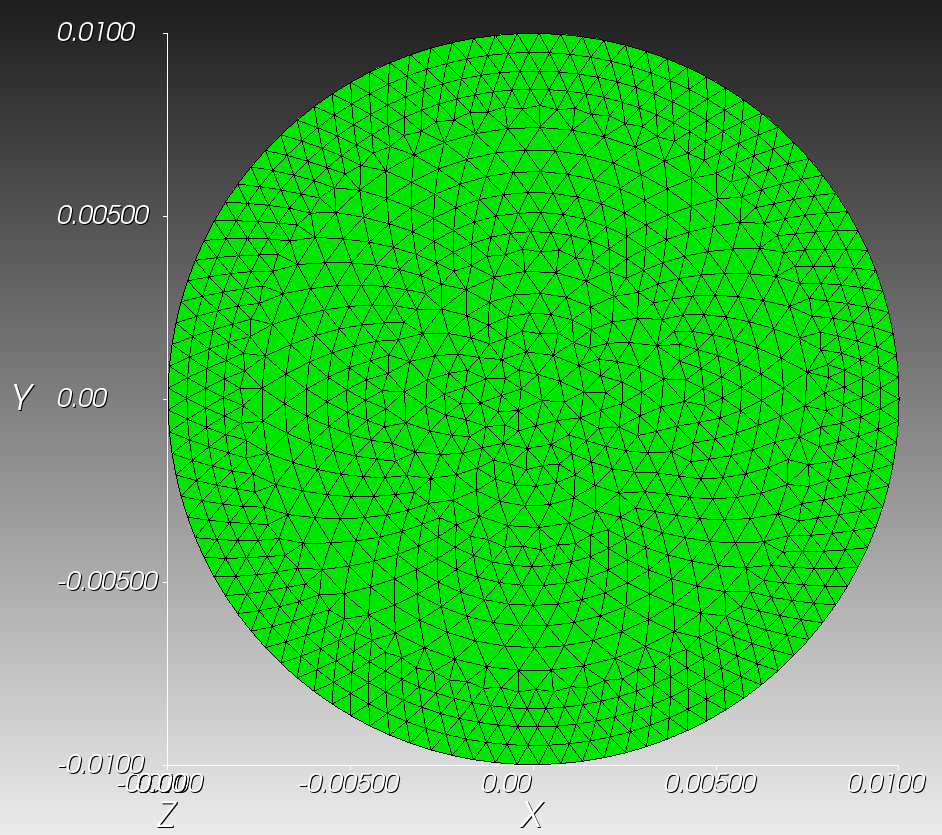
\includegraphics[width=\columnwidth]{circular_mesh.png} 
	\caption{Circular Waveguide Mesh used in Section \ref{subsec:circ_guides}}
	\label{fig:circular_guide}
\end{figure}

\begin{figure}[h!]  
	\centering
	%the command within the [] sets the width of the figure, stability-condition is the jpg name
	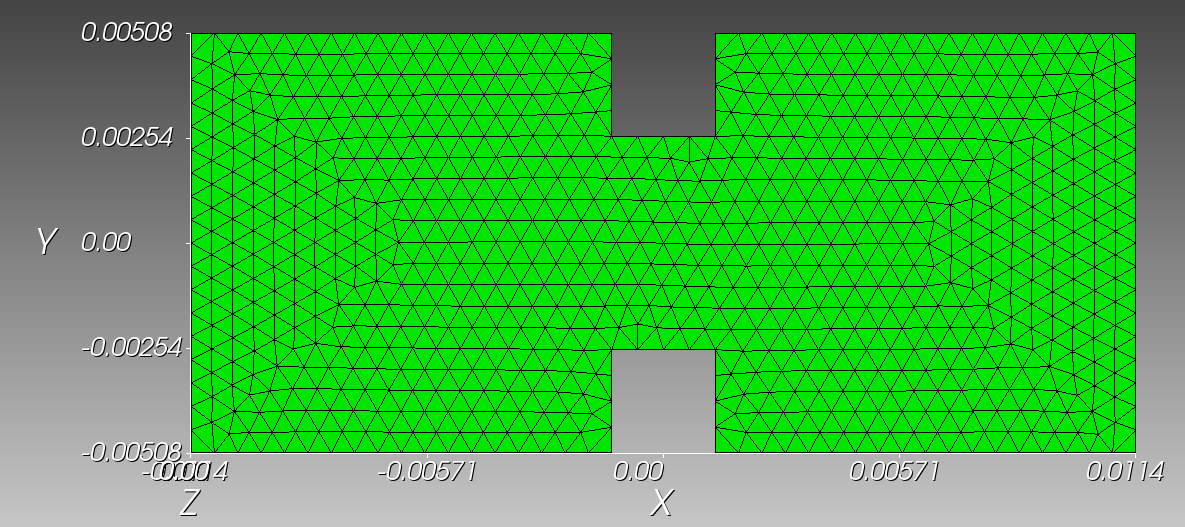
\includegraphics[width=\columnwidth]{ridged_mesh.png} 
	\caption{Ridged Rectangular Waveguide Mesh used in Section \ref{subsec:rid_guides}}
	\label{fig:ridged_guide}
\end{figure}

The mathematical model outlined in Section \ref{sec:mathmod} was implemented in Python for its general flexibility and existing numerical packages such as NumPy and SciPy which were used to solve the general eigenvalue problems established in (\ref{eq:te_eig}-\ref{eq:tm_eig}). In addition to these packages, the MeshIO package was used as it has a built in reader for \verb|.inp| files, allowing mesh data to be read in with ease. From this, all generated data was directly plotted using Matplotlib thereby eliminating the need to save any generated data to disk.

\subsection{Verification and Validation}
\label{subsec:vv}
Prior to performing any kind of `novel' analysis, the implemented model must first be benchmarked against analytic results. For this reason, the case of a WR-90, X-band waveguide with $a=0.02286$m and $b=0.01016$m is first considered \cite{everythingrf}. 

In this and all following sections the spatial distributions of TE modes will be plotted. Only one mode will be plotted per section as these are merely visual aids in comparison to the dispersion charts which will contain data from the first 3 TE and TM modes. The choice of the given TE mode is entirely arbitrary and was chosen for its post processing simplicity and to ensure adequate comparisons exist in the literature \cite{pozar2011microwave}. The $\mathrm{TE}_{11}$, $H_z$ field distribution can be found in Fig. \ref{fig:rect_prof}. 

\begin{figure}[h!]  
	\centering
	%the command within the [] sets the width of the figure, stability-condition is the jpg name
	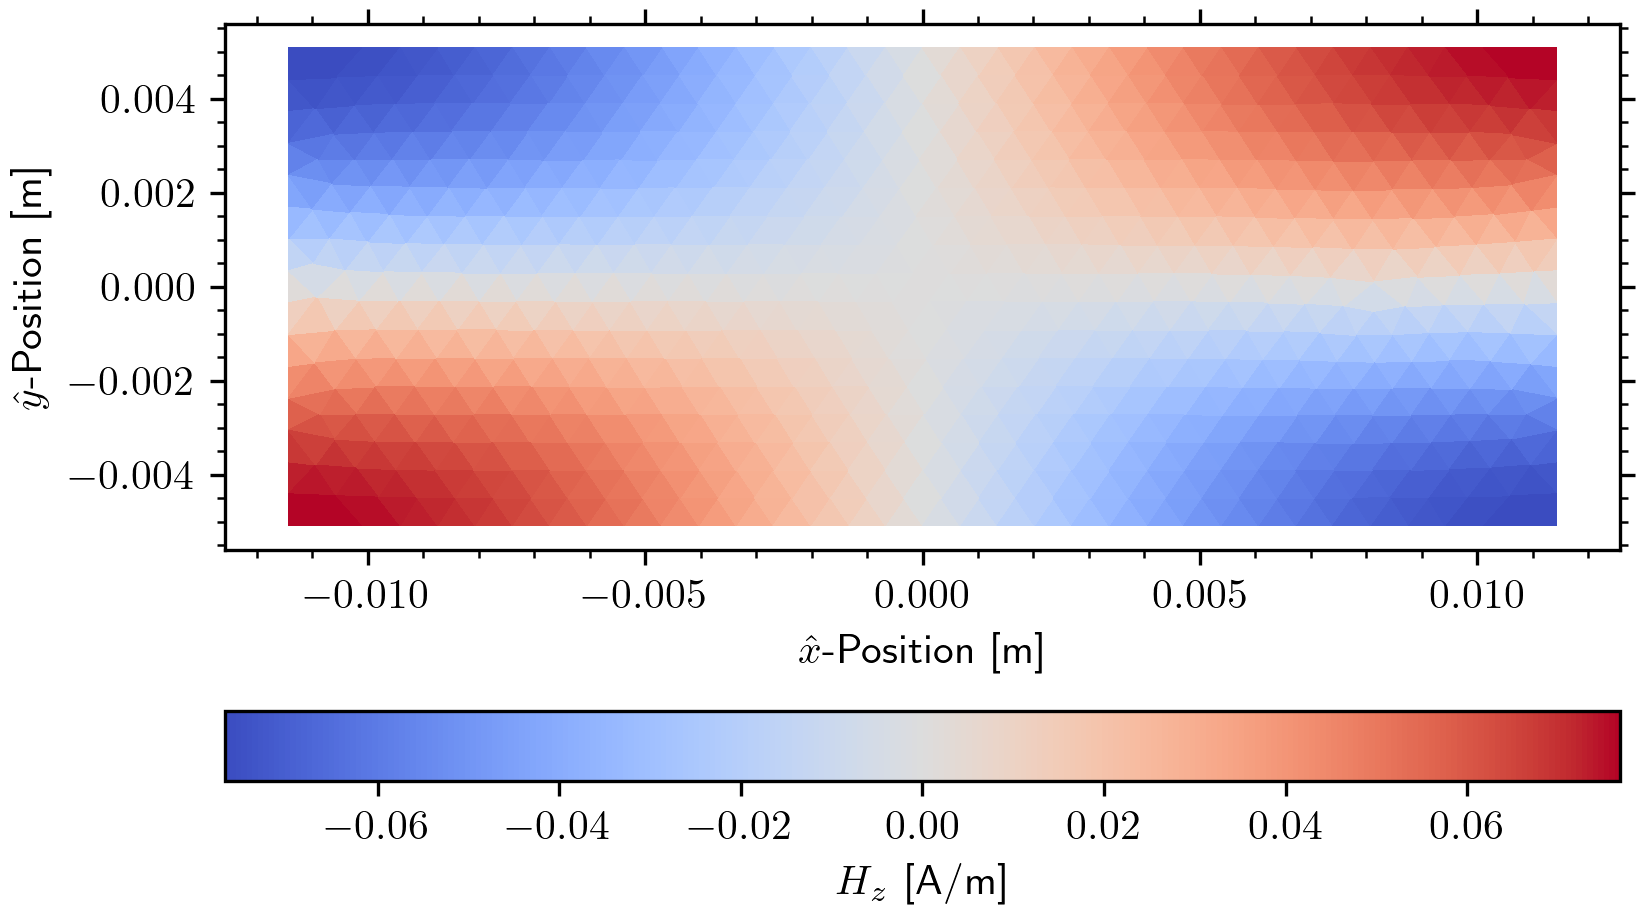
\includegraphics[width=\columnwidth]{te11_rect.png} 
	\caption{$\mathrm{TE_{11}}$, $H_z$ Field Distribution in a Rectangular WR-90, X-band Waveguide}
	\label{fig:rect_prof}
\end{figure}

As seen in Fig. \ref{fig:rect_prof} the $\mathrm{TE_{11}}$, $H_z$ field profile matches that of the $\mathrm{TE}_{11}$ found in the literature \cite{pozar2011microwave} thus confirming its accuracy in recreating spatial field profiles. The $\mathrm{TE}_{10}$ and $\mathrm{TE}_{21}$ modes profiles were also vetted, however are not shown to reduce clutter.

Next, a dispersion plot of the first three TE and TM modes in this waveguide is constructed. To benchmark to theory, the following analytic cutoff wave number is used:
\begin{align}
    k_c=\sqrt{\left(\frac{m\pi}{a}\right)^2+\left(\frac{n\pi}{b}\right)^2},
\end{align}
where $m$ and $n$ are the corresponding mode propagation numbers. From this, the first three, unique, and nonzero simulated cutoff wave numbers from both the TE and TM modes were used to create the dispersion plot in Fig. \ref{fig:rect_disp}.

\begin{figure}[h!]  
	\centering
	%the command within the [] sets the width of the figure, stability-condition is the jpg name
	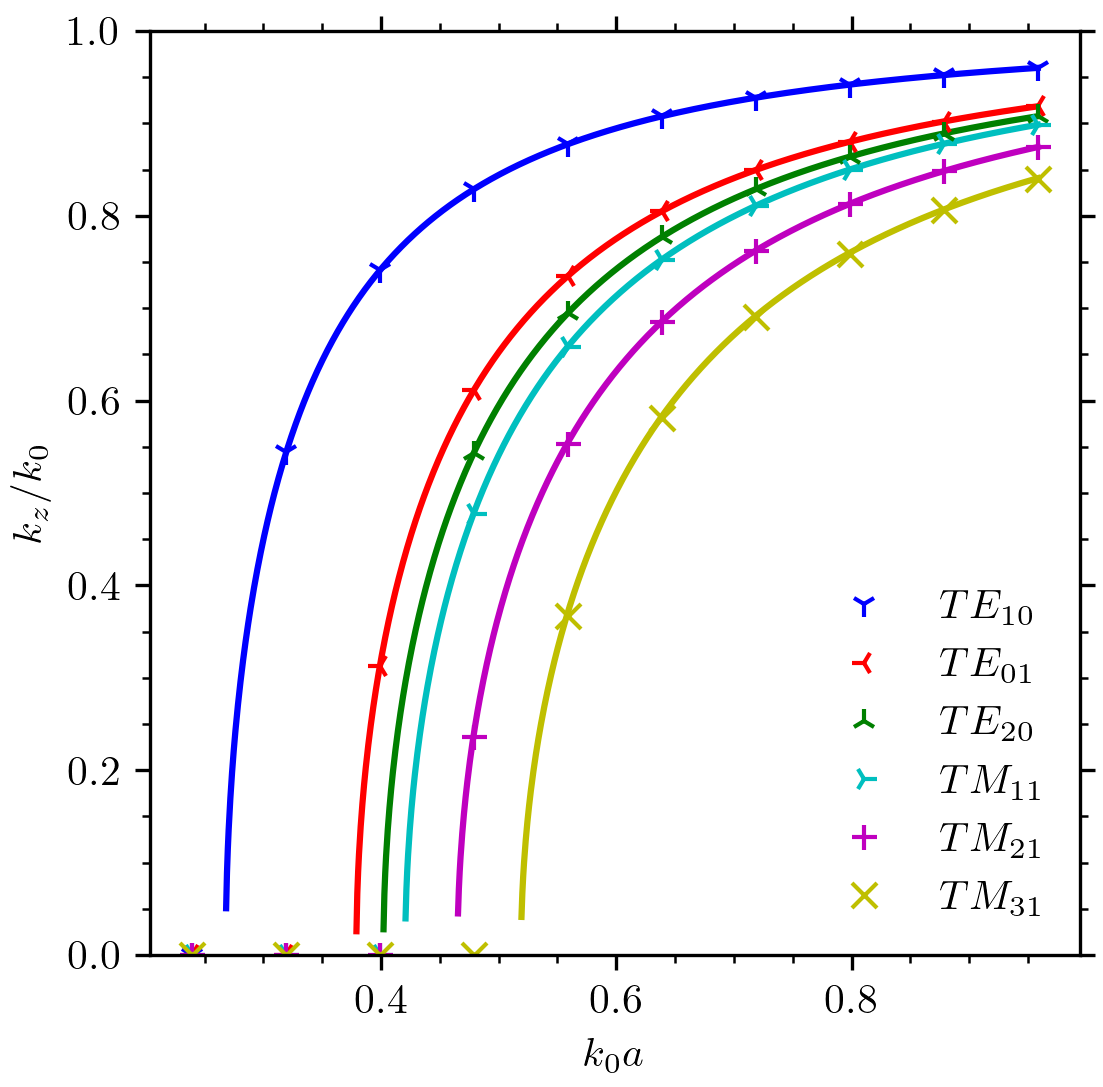
\includegraphics[width=\columnwidth]{rec_waveguide_disp.png} 
	\caption{Dispersion Plots of First Three TE and TM Modes in Rectangular WR-90, X-band Waveguide with Solid Lines as Analytical Results and Corresponding Markers as Simulated Results}
	\label{fig:rect_disp}
\end{figure}

As seen in Fig. \ref{fig:rect_disp}, the dispersion relations predicted by the implemented model match that predicted by theory excellently. Additionally, this demonstrates that the choice of using $\approx2000$ nodes to represent these geometries is more than sufficient to ensure convergence on the true solution. With this, more sophisticated waveguides can now be investigated knowing that the underlying mathematical model is sound.


\subsection{Circular Waveguides}
\label{subsec:circ_guides}
With the model successfully validated against the analytic results of a rectangular waveguide, a circular waveguide of radius $r=0.01$m is now assessed. One last visual verification step is performed by comparing the field profiles of the $\mathrm{TE}_{01}$ and $\mathrm{TE}_{11}$ modes generated by the model to that of the analytic profiles found in literature. The simulated $\mathrm{TE}_{01}$ $H_z$ profile can be found in Fig. \ref{fig:circ_prof}.

\begin{figure}[h!]  
	\centering
	%the command within the [] sets the width of the figure, stability-condition is the jpg name
	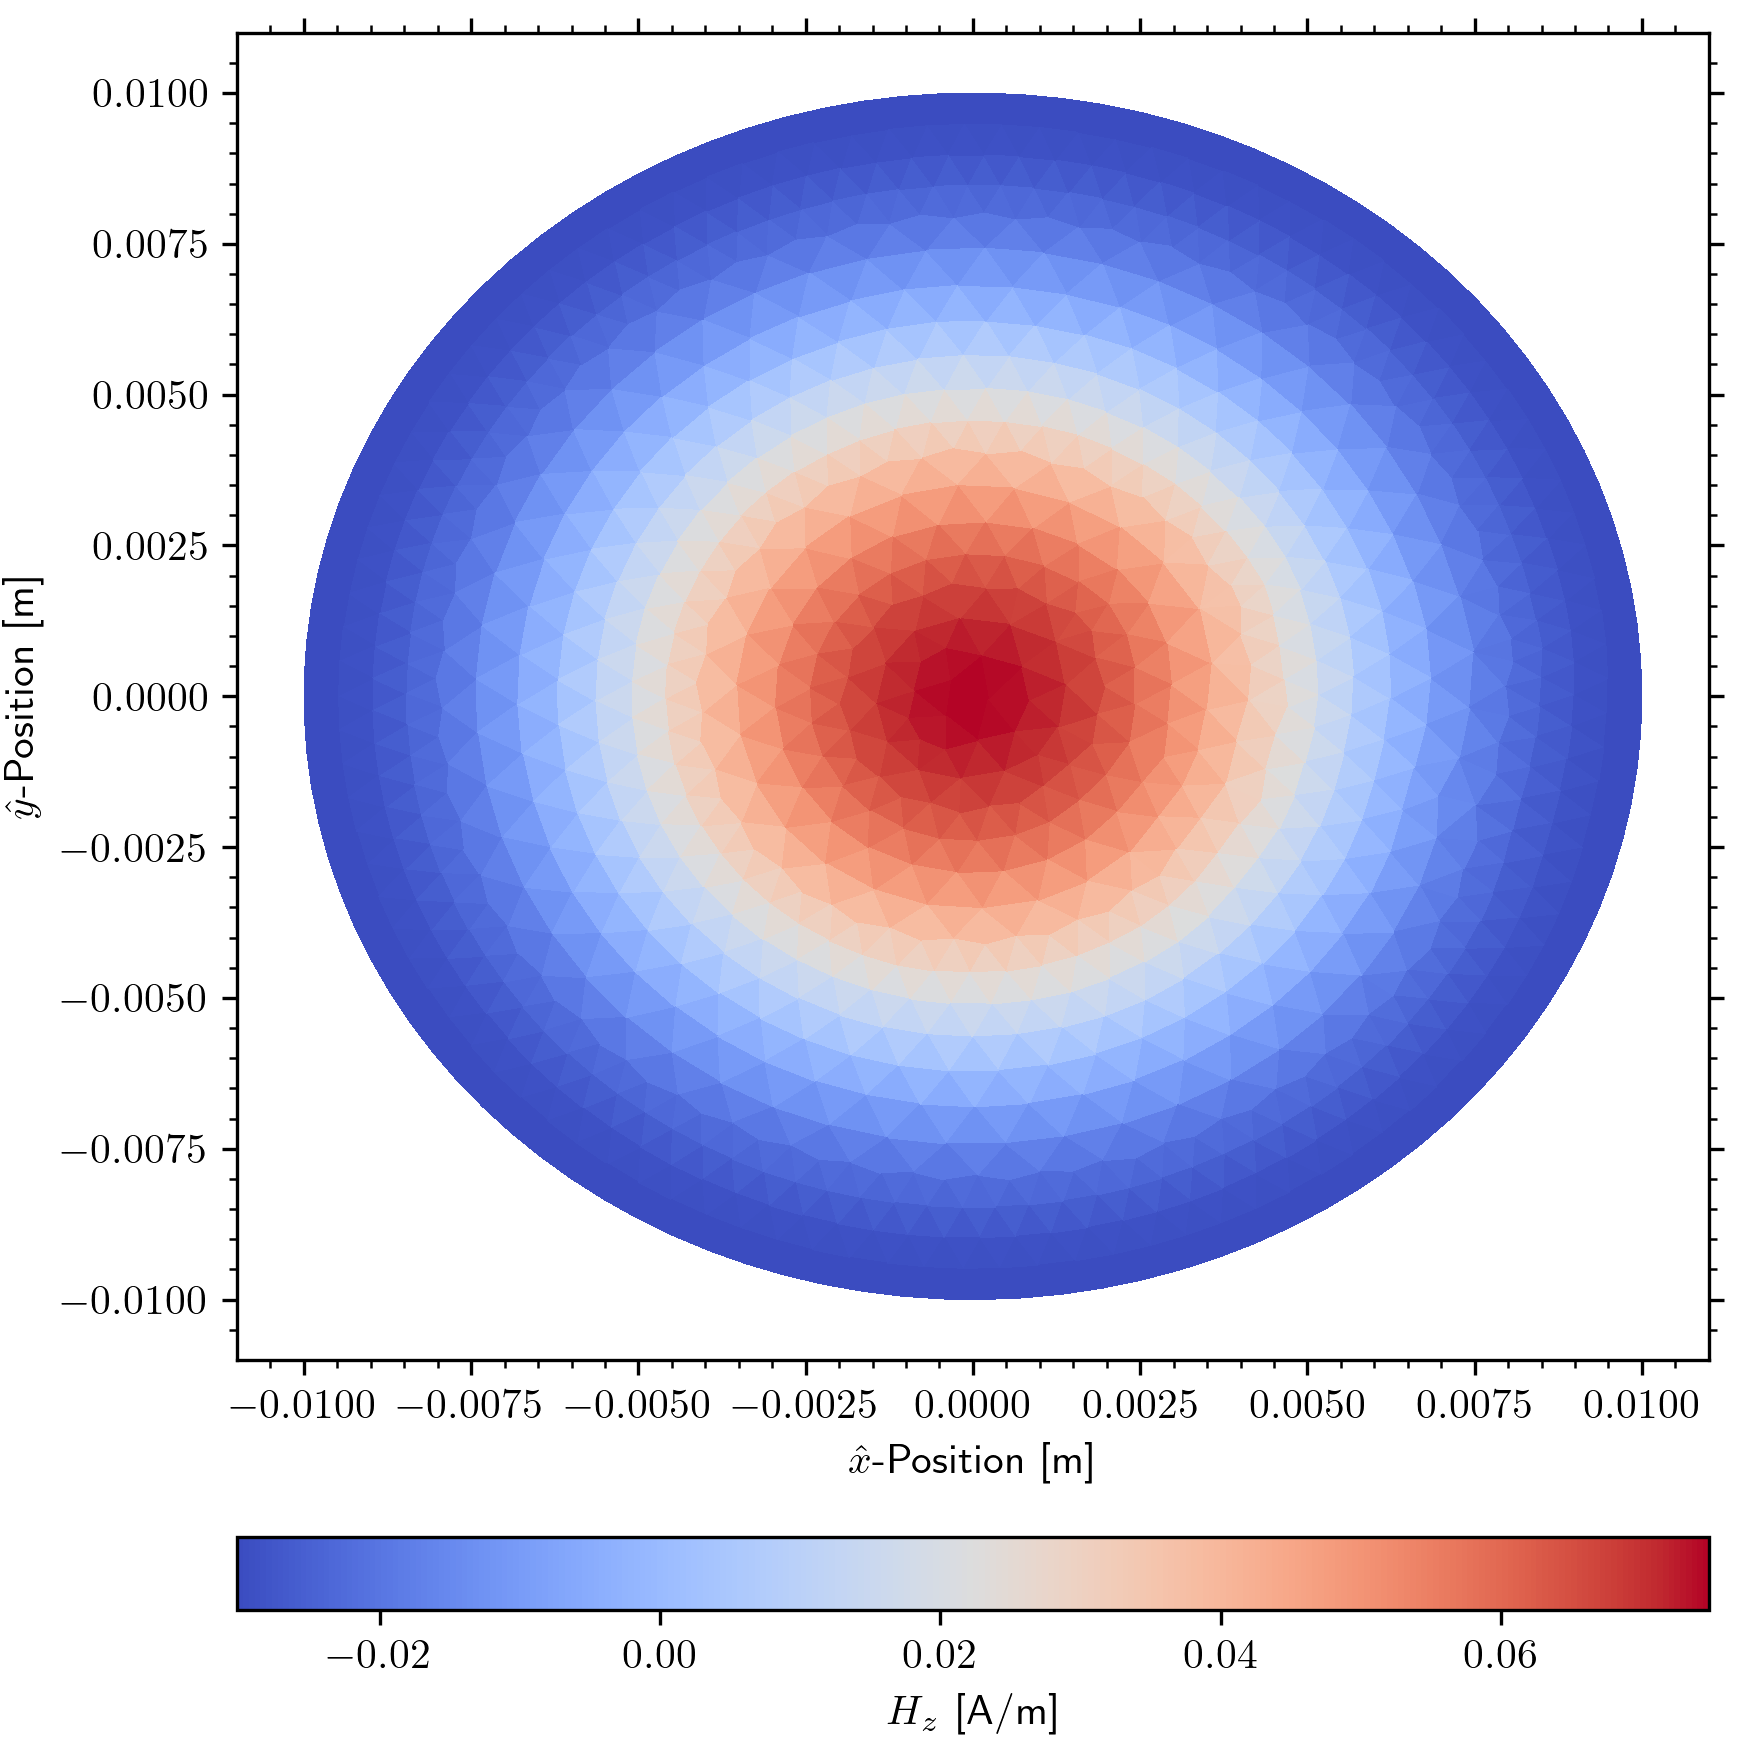
\includegraphics[width=\columnwidth]{te01_circ.png} 
	\caption{$\mathrm{TE_{01}}$, $H_z$ Field Distribution in a Circular Waveguide with $r=0.01$m}
	\label{fig:circ_prof}
\end{figure}

As seen in Fig. \ref{fig:circ_prof}, the $H_z$ profile matches that found in the literature \cite{pozar2011microwave}, thereby providing additional validation for the implemented numerical model. These field plots also highlight one of the main strengths of FEM; which is its ability to work with unstructured grids out of the box. Modeling a similar profile using a finite difference method would result in egregious stair-stepping error if performed in Cartesian coordinates, or would require a special derivation in polar or cylindrical coordinates potentially limiting the model's usefulness. On the other hand, FEA is able to handle these curved geometries using unstructured grids with relative ease. 

From here a similar analysis to that of Fig. \ref{fig:rect_disp} is performed for circular waveguides. Traditionally, producing such plots would require tables containing roots of the Bessel function of the first kind $p_{nm}$ and it's derivative $p^{'}_{nm}$ which are used to determine the cutoff wave numbers as
\begin{align}
	k_c = \frac{p^{'}_{nm}}{r},
\end{align}
and
\begin{align}
	k_c = \frac{p_{nm}}{r}
\end{align}
respectfully for the TE and TM modes \cite{pozar2011microwave}. Using the above FEM, we are able to directly calculate the dispersion relations for any circular waveguide without the use of the roots of a Bessel function or its derivative. The simulated dispersion relations can be found in Fig. \ref{fig:circ_disp}.

\begin{figure}[h!]  
	\centering
	%the command within the [] sets the width of the figure, stability-condition is the jpg name
	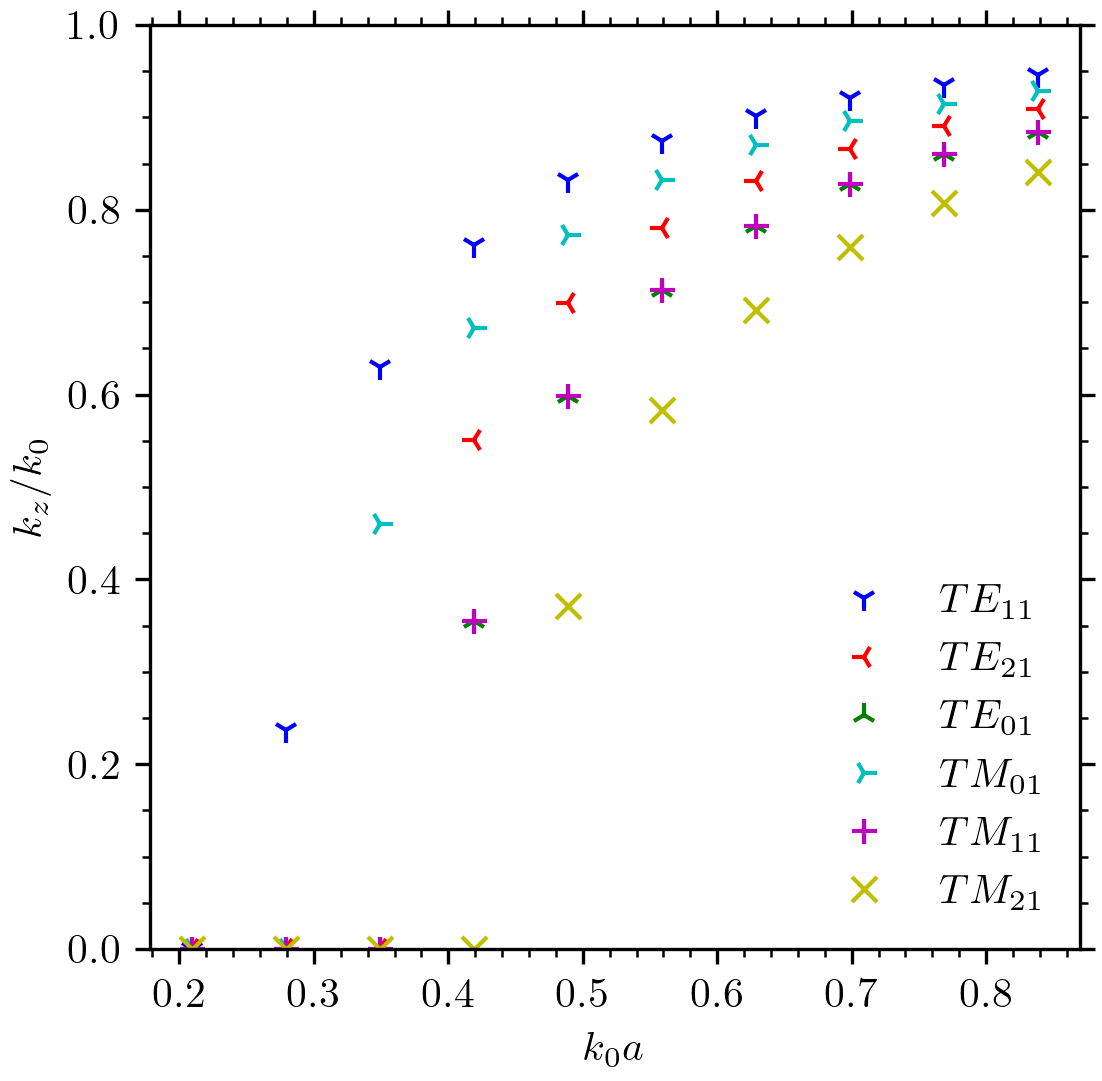
\includegraphics[width=\columnwidth]{circ_waveguide.png} 
	\caption{Dispersion Plots of First Three TE and TM Modes in a Circular Waveguide with $r=0.01$m}
	\label{fig:circ_disp}
\end{figure}

As seen in Fig. \ref{fig:circ_disp}, the bandwidth between individual propagation modes in a circular waveguide is much less than that of rectangular waveguides as shown in Fig. \ref{fig:rect_disp}. This is perhaps most notable between the $\mathrm{TE}_{11}$ dominant mode and the next $\mathrm{TM}_{01}$ mode, which is rather small. This is well documented in the literature \cite{cadencecircular} and is one of the main factors limiting circular waveguides from being used in wide-band applications. Finally, FEA was able to successfully predict the equivalence of the cutoff wave number for the  $\mathrm{TE}_{01}$ and $\mathrm{TM}_{11}$ modes which is well documented in the literature \cite{pozar2011microwave} thereby providing one last verification step prior to considering ridged rectangular waveguides.

\subsection{Comparison of Ridged and Non-Ridged Waveguides}
\label{subsec:rid_guides}
With all validation steps completed, a comparison of a standard WR-90, X-band waveguide to that of a double ridged WR-90, X-band waveguide is now provided. As seen in Fig. \ref{fig:ridged_guide}, ridges are of size $0.0025\times0.0025$m and are placed at the centerline of the waveguide. Similarly to Section \ref{subsec:vv},the $H_z$ field profile of the $\mathrm{TE_{11}}$ mode is assessed as shown in Fig. \ref{fig:rid_prof}.

\begin{figure}[h!]  
	\centering
	%the command within the [] sets the width of the figure, stability-condition is the jpg name
	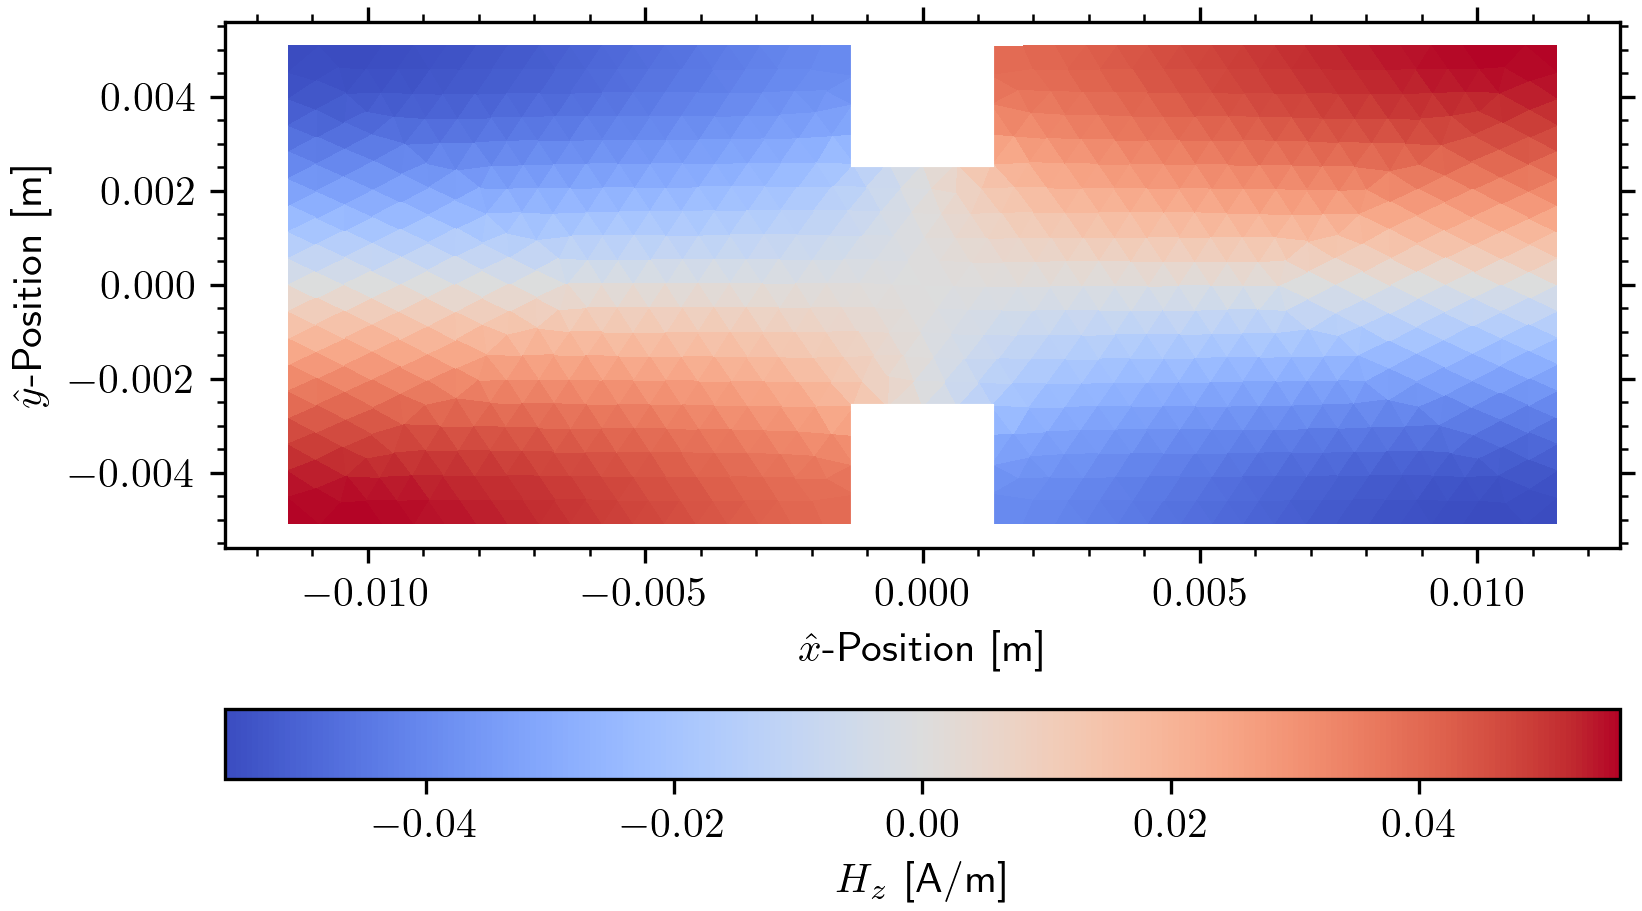
\includegraphics[width=\columnwidth]{te11_rid.png} 
	\caption{$\mathrm{TE_{11}}$, $H_z$ Field Distribution in a Ridged Rectangular WR-90, X-band Waveguide}
	\label{fig:rid_prof}
\end{figure}

As seen in Fig. \ref{fig:rid_prof} the field profile is nearly identical to that of the non-ridged WR-90 waveguide shown in Fig. \ref{fig:rect_prof}. This is expected as the propagation mode is identical despite the introduction of ridges. To demonstrate differences, a dispersion plot for this ridged waveguide is provided. To highlight discrepancies between the ridged and base waveguides, the theoretical base dispersion curves are plotted as solid lines, and the corresponding simulated data for the same modes as markers. Said plot can be found in Fig. \ref{fig:rid_disp}.

\begin{figure}[h!]  
	\centering
	%the command within the [] sets the width of the figure, stability-condition is the jpg name
	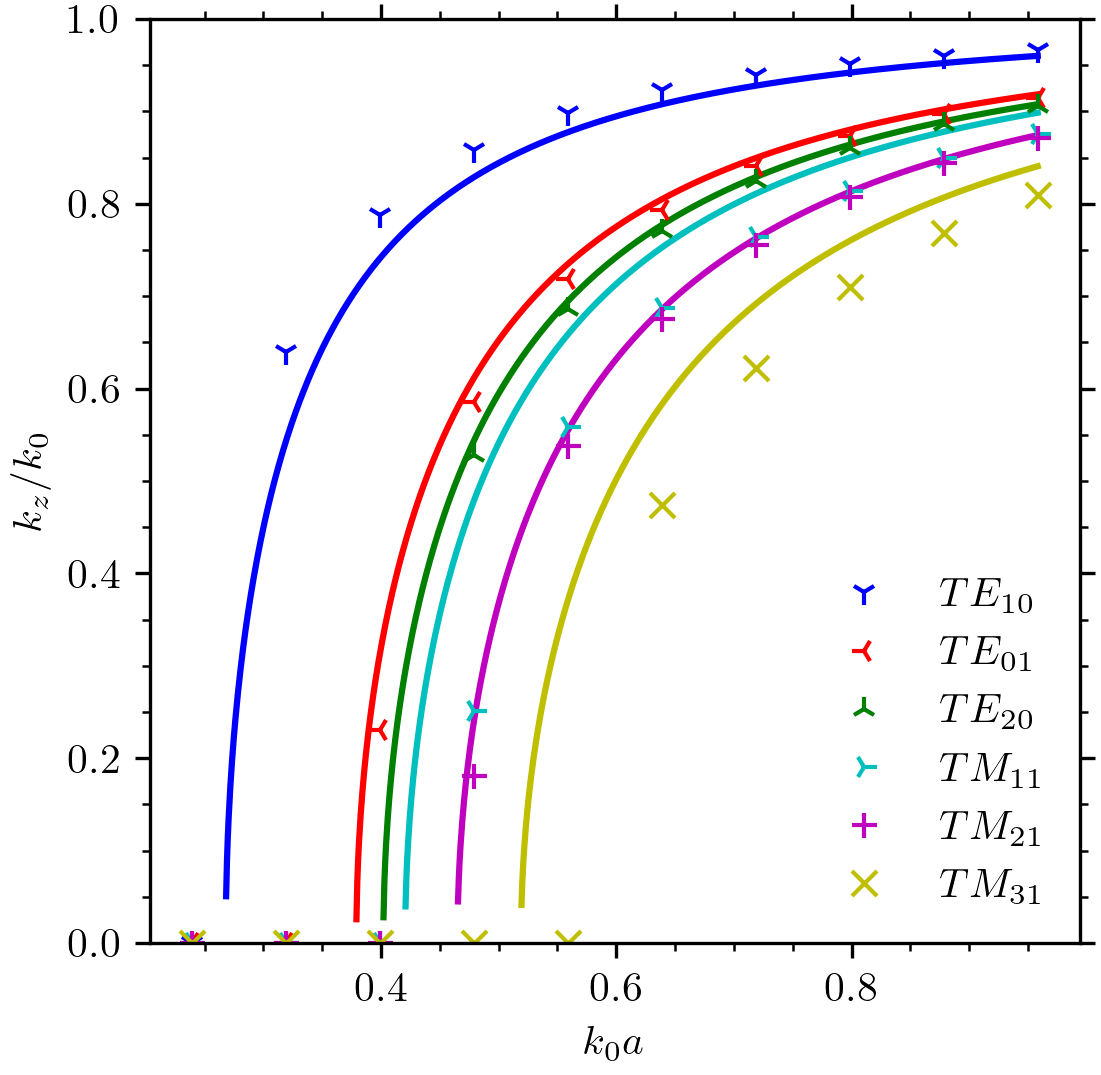
\includegraphics[width=\columnwidth]{ridged_waveguide_w_comp} 
	\caption{$\mathrm{TE_{11}}$, $H_z$ Field Distribution in a Ridged Rectangular WR-90, X-band Waveguide with Solid Lines as the Theoretical Dispersion Relation for Base Waveguide and Corresponding Markers as Simulated Dispersion Relation for Ridged Waveguide}
	\label{fig:rid_disp}
\end{figure}

It is clear from Fig. \ref{fig:rid_disp} that the cutoff wave number of the dominant $\mathrm{TE}_{10}$ mode is less than that of the rectangular waveguide in alignment with the theory \cite{pozar2011microwave}. In addition to this, all fields with cutoff wave numbers greater than the dominant mode all experience an increase in cutoff wave number within the ridged waveguide. These phenomenon can all be explained via field buckling caused by the inclusion of ridges. To demonstrate this, the field profiles of the dominant $\mathrm{TE}_{10}$ modes for both the base and ridged waveguides are plotted which can be found in Figs. \ref{fig:rec_te10}-\ref{fig:rid_te10}.

\begin{figure}[h!]  
	\centering
	%the command within the [] sets the width of the figure, stability-condition is the jpg name
	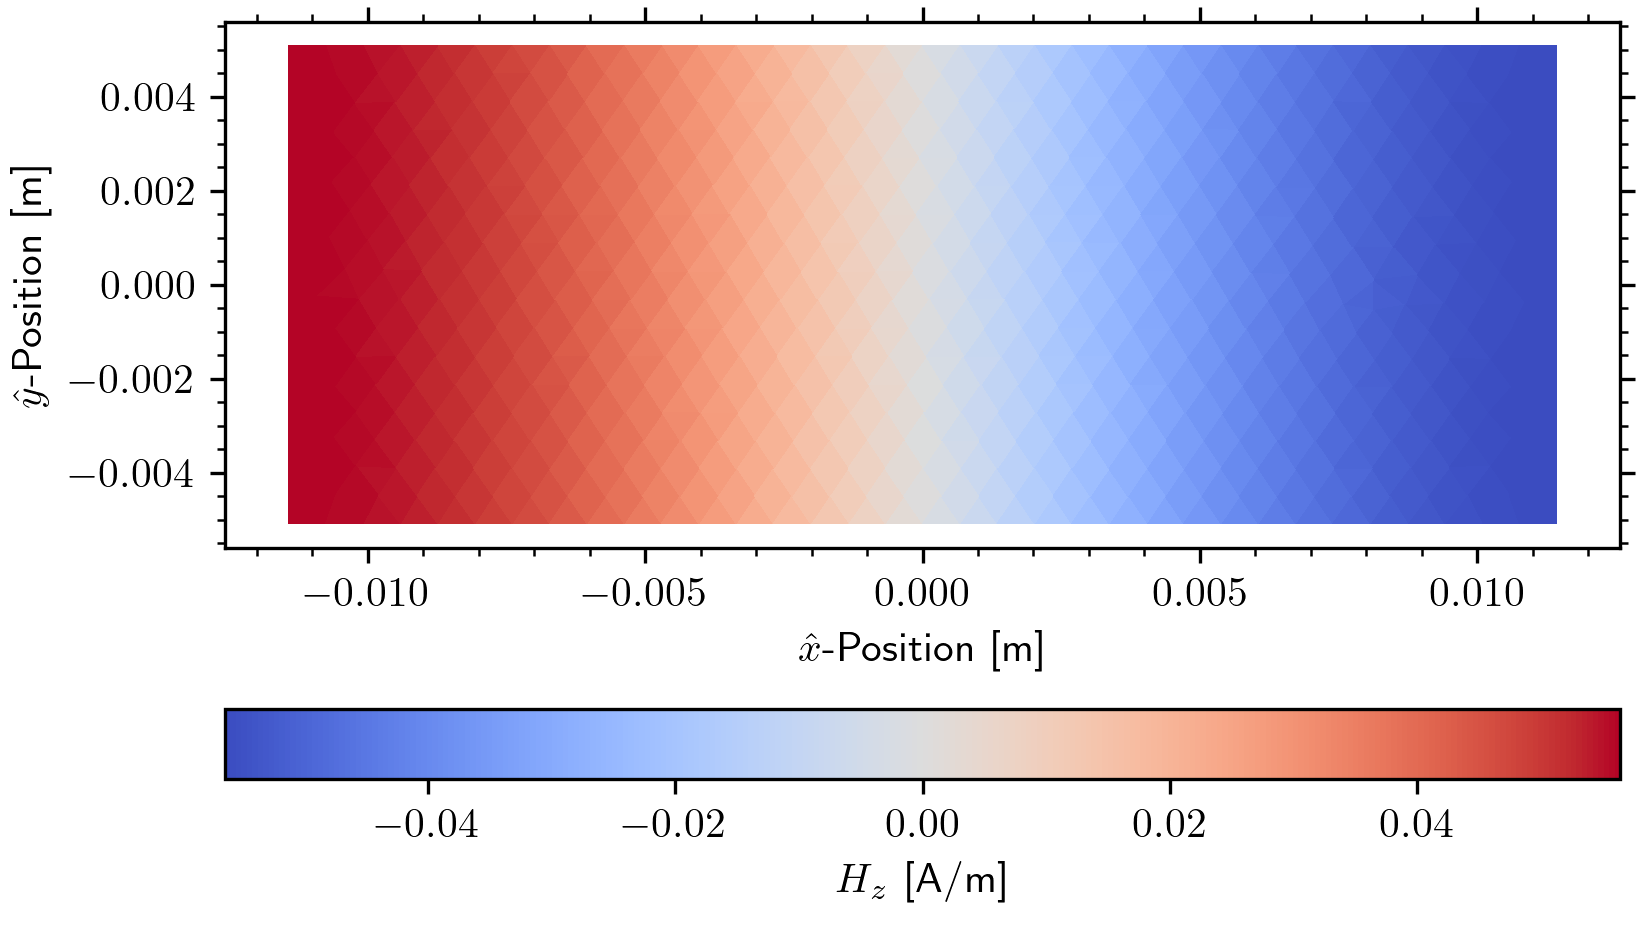
\includegraphics[width=\columnwidth]{te10_rect.png} 
	\caption{Dominant $\mathrm{TE_{10}}$, $H_z$ Field Distribution in a Rectangular WR-90, X-band Waveguide}
	\label{fig:rec_te10}
\end{figure}

\begin{figure}[h!]  
	\centering
	%the command within the [] sets the width of the figure, stability-condition is the jpg name
	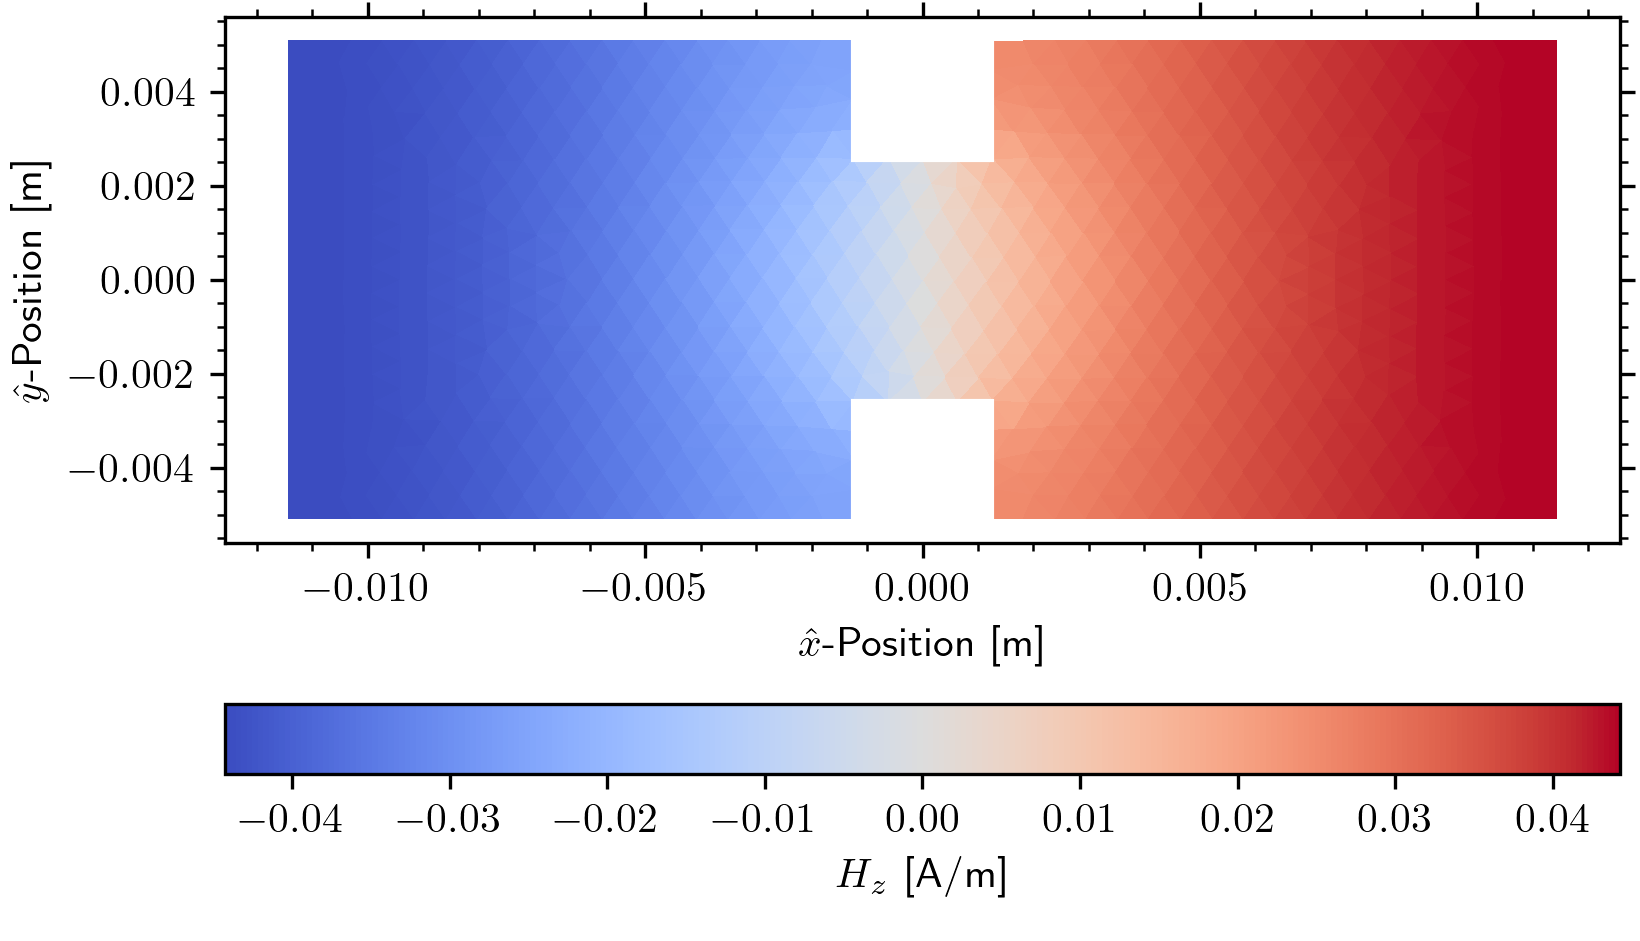
\includegraphics[width=\columnwidth]{te10_ridged.png} 
	\caption{Dominant $\mathrm{TE_{10}}$, $H_z$ Field Distribution in a Ridged Rectangular WR-90, X-band Waveguide}
	\label{fig:rid_te10}
\end{figure}

Fig. \ref{fig:rec_te10} shows that in the base waveguide there are two distinct regions within the $\mathrm{TE}_{10}$, $H_z$ field profile. In the case of the ridged waveguide, the ridges align with the gap between these field regions allowing for the same field profile to be achieved at lower frequencies, thus resulting in the lowering of the cutoff wave number. In other words, the inclusion of ridges facilitates a lower overall field buckling for this propagation mode. In contrast to this, higher order modes such as the $\mathrm{TE}_{11}$ mode found in Fig. \ref{fig:rid_prof} require increased buckling in order to satisfy the boundary conditions of (\ref{eq:diriclet_tm}-\ref{eq:neumann_te}) to achieve the same field profile. This increased field buckling directly corresponds to an increase in the minimum cutoff wave number, and corresponding frequency content, to recreate these higher-order, more complex, propagation modes. For this reason, ridged waveguides offer superior bandwidth for the dominant modes making them superior for transmitting high-bandwidth signals.   

\section{Conclusion}
\label{sec:conclusion}
A 2-dimensional method of moments program was developed from Maxwell's Equations allowing for the charge distribution to be calculated on an arbitrarily sized square metallic plate for an arbitrary number of elements per side. The charge distribution was then integrated to find the total charge collected on the metallic plate. Finally, the total charge was then used to solve for the capacitance of the plate given an arbitrary applied equipotential. These predicted capacitances were next verified against those obtained from Monte Carlo methods found in the literature of which they agreed well. The charge distribution as a function of space was then analyzed and explained with basic electrostatic theory. Finally, a convergence study was performed and showed that all methodologies tested converge to a predicted capacitance of approximately $0.4075$pF and all predict values within $0.1\%$ of eachother for $n\geq30$.

While relatively general in the sense that the model works for any side length, applied potential, and number of elements per side, this model is not performant. Upon software profiling, it was discovered that the code spends the majority of its run time assembling the matrices. This is most notable in the exact square element, and subdomain collocation procedures where each element of the system matrix takes between $4-16$ iterations to fully assemble. When combined with the Python's abysmal loop performance, the matrix assembly dominates the program execution time. To that end, future work should first focus rewriting the model in a language like C/C++/Rust, all of which have optimizing compilers that can take advantage of loop unrolling to dramatically speed up the assembly process. After which, the next logical step would be to expand support to handle unstructured meshes such that the capacitance of arbitrary shaped surfaces could be obtained.
%\section{Appendix}
\label{sec:Appendix}

\subsection{Code Structure}
\label{subsec:code}
Code is broken up into logical modules, as is custom in Rust, which contain related aspects of the code. The file \verb|./src/main.rs| contains the `main' function that is built into a binary. The file \verb|./src/solver.rs| contains a high level interface for interacting with and bootstrapping the simulation. The file \verb|./src/geometry.rs| contains a structure that holds information relevant to the geometry of the simulation. Finally, the \verb|./src/engine.rs| contains all data and methods needed to evolve the simulation in time and contains much of the simulation code. All functions are commented using function comments in the source code which are automatically assembled into an interactive webpage containing all project documentation. Said documentation can be found under the \verb|./doc/| directory. As such project documentation can either be viewed by looking at the source code and/or viewing the interactive documentation pages by opening \verb|./doc/waveguide/index.html| with a web browser. The code can easily be compiled with cargo (the package manager that comes with Rust much like Pip for Python) using the command \verb|cargo build --release|. The compiled binary can then be executed by running \verb|./target/release/driver.exe|. This binary reads in data from \verb|config.toml| which contains all simulation parameters.


\bibliographystyle{IEEEtran}
\bibliography{cem_class_example_bib} %this should point to your bibliography file.

% that's all folks
\end{document}


